\documentclass{article}
\usepackage{graphicx} % Required for inserting images
\usepackage{amsmath}
\usepackage{tikz}
\usetikzlibrary{shapes.multipart}


\title{Java Project Report \\ Arbitrary Arithmetic Precision}
\author{Gulla Mitra \\ \\CS24BTECH11027}
\date{May 2025}

\begin{document}

\maketitle

\section{Introduction}

This document provides a implementation of Arbitrary precision arithmetic in Java. The main motivation for this project is to overcome the limitations of built in numeric types which cannot handle large inputs as size is bounded. By representing numbers as strings we can perform fundamental arithmetic operations manually, this approach provides full control over precision, sign handling.\\

The system includes support for both integer and floating point operations,organized into 
seperate classes: \textbf{AInteger}, \textbf{AFloat}, to execute operations.There is main class \textbf{MyInfArith} which handles command line arguments and perform required arithmetic operations.\\

Operations Addition,Subtraction,Mutiplication,Divison can be performed in both integer and float types. \\

\section{Project Folder}

\begin{verbatim}
    project_folder-
                    javasrc-
                            arbitraryarithmetic-
                                                AInteger.java
                                                AInteger.class
                                                AFloat.java
                                                AFloat.class
                            MyInfArith.java
                            MyInfArith.class

                            
                    build-
                          arbitraryarithmetic-
                                              AInteger.class
                                              AFloat.class
                          MyInfArith.class
                    arbitraryarithmetic-
                                        aarithmetic.jar
                    build.xml
                    execute_java.py
                    latex_report.pdf
                    latex_report.tex
                    
\end{verbatim}

\section{AInteger.java}

The \texttt{AInteger} class provides functionality for representing and manipulating arbitrarily large integers using string-based internal storage. It supports arithmetic operations like addition, subtraction, multiplication and division with proper handling of signs.

\subsection*{Constructors}

\begin{itemize}
    \item \texttt{AInteger()} \\
    Default constructor AInteger() that initializes the instance with value "0".

    \item \texttt{AInteger(String str)} \\
    Constructor AInteger(String s) that initializes the instance by the number whose string representation is given by ’s’.Removes leading zeros if present.
    \item \texttt{AInteger(AInteger other)} \\
    Copy constructor that creates an instance of AInteger.
\end{itemize}


\subsection*{Methods}

\begin{itemize}

    \item \textbf{removezeroes(String str)} \\
    This method removes the leading zeroes if present in the string.If zeroes are present while performing operations some Errors may occur.So we should remove zeroes using this method. 

    \item \textbf{Sign(String str1,String str2)} \\
    Determines the sign of the result when subtracting two non-negative integer strings. If \texttt{str1} is less than \texttt{str2}, the method returns \texttt{"-"} indicating result as negative, otherwise, returns an empty string.This method is used in subtraction of two non negative integers.

    \item \textbf{less(String str1, String str2)} \\
    Determines the lesser string in the given two strings.This method is used in division to know which string is lesser in the given two strings.
    
    \item \textbf{parse(String str)} \\
    This static method creates and returns a new \texttt{AInteger} instance initialized with the given string \texttt{str}.
    It is equivalent to calling a constructor with a string.

    \item \textbf{toString()} \\
    Returns the internal string representation of the AInteger object.

    \item \textbf{addition(String str1,String str2)}\\
    Performs digit-wise addition of two non-negative integer strings \texttt{str1} and \texttt{str2}. The method iterates from right to left carrying the carry.\\This logic is same as manual addition. The final result is returned as a string after removing the leading zeroes.

    \item \textbf{subtract(String str1,String str2)} \\
    Performs the digit-wise subtraction of two non-negative integer strings. If first number \texttt{str1} is smaller than \texttt{str2},then the method swaps the two numbers and stores the negative sign. It handles borrowing if needed and returns the result as a string after removing the leading zeroes.

    \item \textbf{multiply(String str1,String str2)} \\
    Performs the digit-wise mutiplication of two non-negative integer strings similar to the manual multiplication.for each digit in the \texttt{str2} starting from right side, it mutiples it with every digit in \texttt{str1} and forms partial products.\\
    These partial products are shifted properly by appending zeroes and are added using \texttt{addition} method.It returns the final result as a string after removing the leading zeroes.

    
    \item \textbf{AInteger add(AInteger other)} \\
    Adds the current \texttt{AInteger} to another instance. It handles the signs of both number strings and determines whether the operation should be an addition or subtraction and calls the required function. Prefixes the correct sign to final result and returns as a new \texttt{AInteger} instance containg sum.

    \item \textbf{AInteger sub(AInteger other)} \\
    Subtracts another \texttt{AInteger} instance from the current one. It handles the signs of both number strings and determines whether the operation should be an addition or subtraction and calls the required function. Prefixes the correct sign to the final result and returns a new \texttt{AInteger} instance containing difference.


    \item \textbf{AInteger mul(AInteger other)} \\
    Multiplies the current \texttt{AInteger} with another instance. This method first checks the signs of both number strings to determine the sign of the final result using \texttt{XOR} logic (XOR-the result is false if exactly one is false). \\
    After checking sign,it removes negative signs if present,then calls \texttt{multiply} method.Prefixes the sign to the final result if needed and returns a new \texttt{AInteger} instance containing the product.

    \item \textbf{AInteger div(AInteger other)} \\
    Divides the current \texttt{AInteger} by another instance and returns the quotient as a new \texttt{AInteger} instance. This method first checks the signs of both number strings to determine the sign of the final result using \texttt{XOR} logic (XOR-the result is false if exactly one is false).After checking for sign it removes negative signs if present.\\ \\
    The division is performed using repeated subtraction. It appends each digit of the dividend from left to right to a temporary string "temp" and when this temp is greater than the divisor then it keeps subtracting the divisor from it as many times as possible. The number of subtractions at each step are added to the quotient which is the final result. Leading zeros are removed from the result before returning.\\ 
    If divisor is zero then the method throws an \texttt{ArithmeticException} to prevent division by zero.
    Prefixes the sign to the final result if needed and returns a new \texttt{AInteger} instance containing the final result.
    
\end{itemize}
\subsection*{UML Diagram for AInteger}

\begin{center}
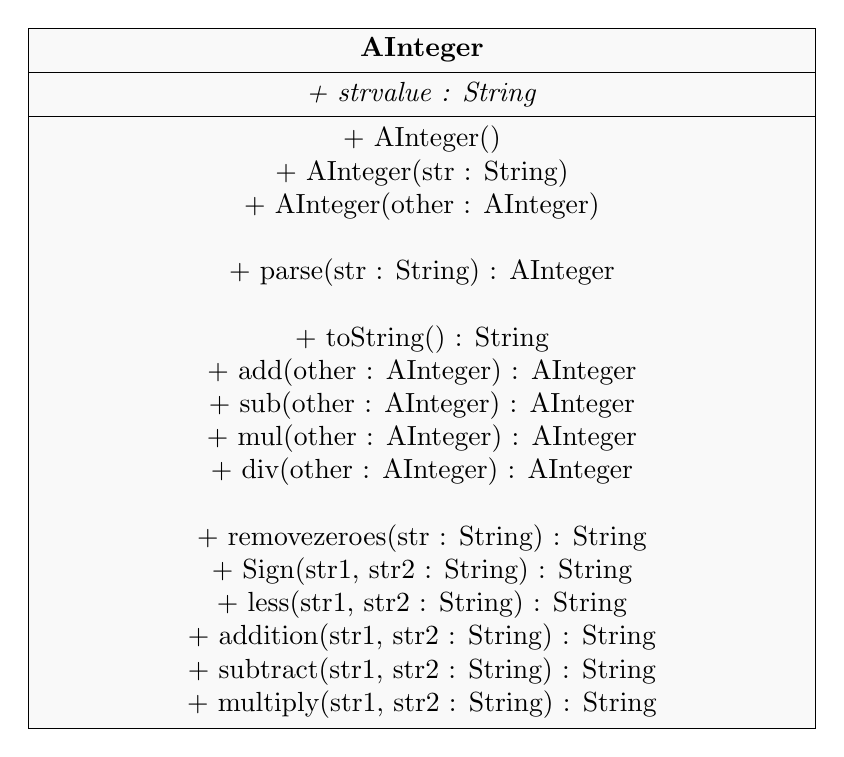
\begin{tikzpicture}
\node[draw, rectangle split, rectangle split parts=3, minimum width=10cm, align=center, fill=gray!5] (AInteger) {
    \textbf{AInteger}
    \nodepart{second}
    \textit{+ strvalue : String}
    \nodepart{third}
    % Constructors
    + AInteger() \\
    + AInteger(str : String) \\
    + AInteger(other : AInteger) \\
    \\
    % Static method
    + parse(str : String) : AInteger \\
    \\
    % Public methods
    + toString() : String \\
    + add(other : AInteger) : AInteger \\
    + sub(other : AInteger) : AInteger \\
    + mul(other : AInteger) : AInteger \\
    + div(other : AInteger) : AInteger \\
    \\
    % Internal helper methods
    + removezeroes(str : String) : String \\
    + Sign(str1, str2 : String) : String \\
    + less(str1, str2 : String) : String \\
    + addition(str1, str2 : String) : String \\
    + subtract(str1, str2 : String) : String \\
    + multiply(str1, str2 : String) : String
};
\end{tikzpicture}
\end{center}

\section{AFloat.java}


The \texttt{AFloat} class provides functionality for representing and manipulating very large floating point numbers with arbitrary precision. It stores the number as a string and supports arithmetic operations like addition, subtraction, multiplication and division with proper handling of signs and decimal places.

\subsection*{Constructors}

\begin{itemize}
    \item \texttt{AFloat()} \\
    Default constructor AFloat() that initializes the instance with value "0".

    \item \texttt{AFloat(String str)} \\
    Constructor AFloat(String s) that initializes the instance by the number whose string representation is given by ’s’.

    \item \texttt{AFloat(AFloat other)} \\
    Copy constructor that creates an instance of AFloat.
    
\end{itemize}

\subsection*{Methods}

\begin{itemize}

    \item \textbf{removezeroesatstart(String str)} \\
    This method removes the leading zeroes if present in the string. If the input number string starts with a decimal point, then "0" is added before the point.

    \item \textbf{removezeroesatend(String str)} \\
    This method removes unnecessary trailing zeroes after the decimal point. If all digits after decimal point are zero,then one zero is added after the decimal.

    \item \textbf{Sign(String str1,String str2)} \\
    Determines the sign of the result when subtracting two non-negative floating point strings. If \texttt{str1} is less than \texttt{str2}, then the method returns \texttt{"-"} indicating result as negative, otherwise returns an empty string. This method is used in subtraction.

    \item \textbf{less(String str1, String str2)} \\
    Determines the lesser string in the given two. This method is used in division to know which string is lesser in the given two strings.

    \item \textbf{decimalindex(String str)} \\
    This method returns the decimal point index in the string. If decimal is not present it returns the length of string.

    \item \textbf{addzeroes(int index, String str)} \\
    If decimal is not present in the string, this method appends ".0" to the string.

     \item \textbf{thirtydecimals(String str)} \\
    This method truncates the decimal part to at most 30 digits after decimal point and returns the result string.

    \item \textbf{parse(String str)} \\
    This static method creates and returns a new \texttt{AFloat} instance initialized with the given string \texttt{str}. It is equivalent to calling a constructor with a string.

    \item \textbf{toString()} \\
    Returns the internal string representation of the AFloat object.

    \item \textbf{addition(String str1,String str2)} \\
    Performs digit-wise addition of two non negative integer strings which are aligned properly. The method iterates from right to left carrying the carry.\\This logic is same as manual addition. The final result is returned as a string after removing the leading zeroes.

    \item \textbf{subtract(String str1,String str2)} \\
    Performs the digit-wise subtraction of two non-negative integer strings. If first number \texttt{str1} is smaller than \texttt{str2},then it swaps the two numbers and stores the negative sign. It handles borrowing if needed and returns the result as a string after removing the leading zeroes.

    \item \textbf{multiply(String str1,String str2)} \\
    Performs the digit-wise multiplication of two numeric strings. For each digit in \texttt{str2} starting from right, it multiplies with every digit in \texttt{str1} and forms partial products. These partial products are shifted properly by appending zeroes and added using \texttt{addition} method. It returns final result as a string after removing the leading zeroes.

    \item \textbf{AFloat add(AFloat other)} \\
    Adds the current \texttt{AFloat} to another instance. It aligns the decimals of both numbers and determines whether the operation should be an addition or subtraction based on the signs of two numeric strings and calls the required function.Adds the decimal correctly to the string in the correct position.Prefixes the correct sign to final result and returns as a new \texttt{AFloat} instance containing sum with 30 digits after decimal.

    \item \textbf{AFloat sub(AFloat other)} \\
    Subtracts another \texttt{AFloat} instance from the current one. It aligns the decimals and handles the signs of both strings. Determines whether to call addition or subtraction based on the signs of two numbers.Adds the decimal correctly to the string in the correct position. Prefixes the correct sign to the final result and returns a new \texttt{AFloat} instance containing difference with 30 digits after decimal.

    \item \textbf{AFloat mul(AFloat other)} \\
    Multiplies the current \texttt{AFloat} with another instance. This method removes the decimal points, performs multiplication using \texttt{multiply} method, and then re-inserts the decimal at the correct position. Sign is handled using \texttt{XOR} logic. Prefixes the sign to the final result if needed and returns the result as a new \texttt{AFloat} instance containing product with 30 digits after decimal.

    \item \textbf{AFloat div(AFloat other)} \\
    Divides the current \texttt{AFloat} by another instance and returns the quotient as a new \texttt{AFloat} instance. It removes the decimal points and balances the digits after decimal. Division is performed using repeated subtraction logic similar to integer division. It adds precision up to 30 decimal places. If divisor is zero then method throws an \texttt{ArithmeticException} to prevent division by zero.

\end{itemize}
    
  \begin{center}
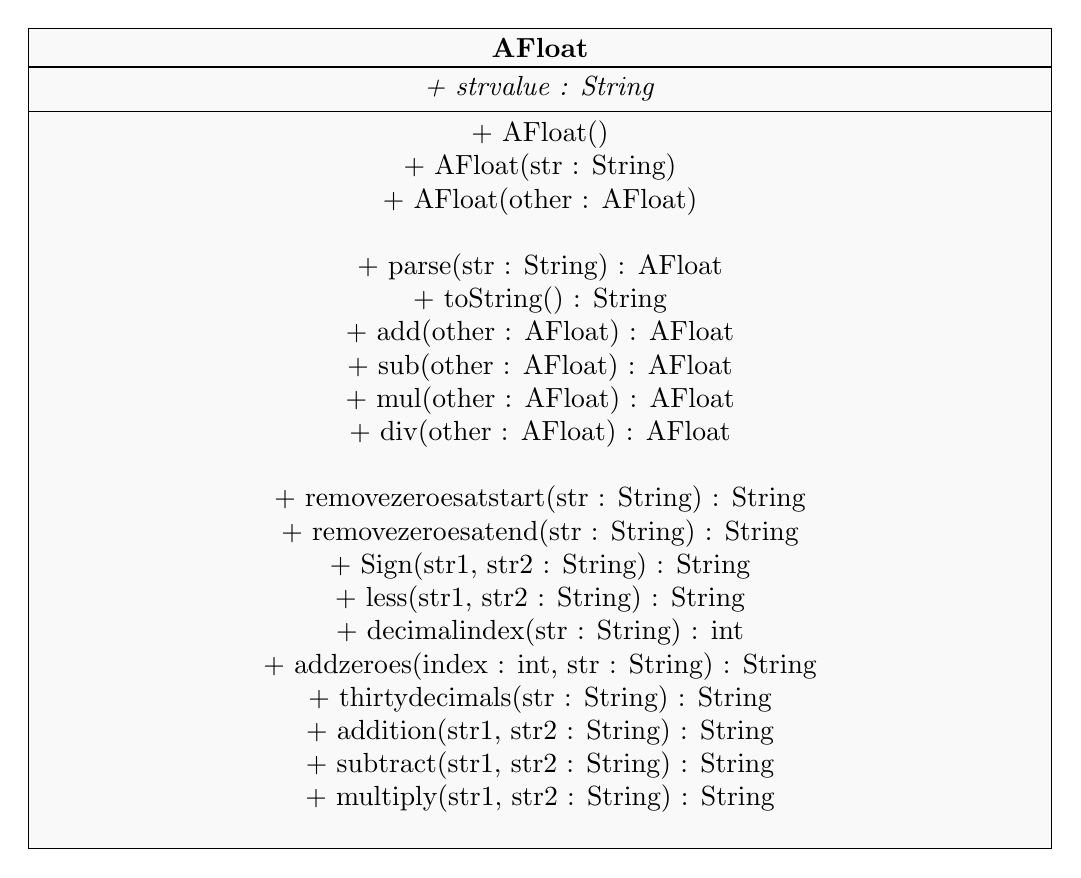
\begin{tikzpicture}
\node[draw, rectangle split, rectangle split parts=3, minimum width=13cm, align=center, fill=gray!5] (AFloat) {
    \textbf{AFloat}
    \nodepart{second}
    \textit{+ strvalue : String}
    \nodepart{third}
    % Constructors
    + AFloat() \\
    + AFloat(str : String) \\
    + AFloat(other : AFloat) \\
    \\
    % Static and public methods
    + parse(str : String) : AFloat \\
    + toString() : String \\
    + add(other : AFloat) : AFloat \\
    + sub(other : AFloat) : AFloat \\
    + mul(other : AFloat) : AFloat \\
    + div(other : AFloat) : AFloat \\
    \\
    % Internal helper methods
    + removezeroesatstart(str : String) : String \\
    + removezeroesatend(str : String) : String \\
    + Sign(str1, str2 : String) : String \\
    + less(str1, str2 : String) : String \\
    + decimalindex(str : String) : int \\
    + addzeroes(index : int, str : String) : String \\
    + thirtydecimals(str : String) : String \\
    + addition(str1, str2 : String) : String \\
    + subtract(str1, str2 : String) : String \\
    + multiply(str1, str2 : String) : String \\
};
\end{tikzpicture}
\end{center}

\section{MyInfArith.java}

The \texttt{MyInfArith} class contains the \texttt{main()} method and acts as the entry point for the program. It is responsible for taking input arguments from the command line and calling the appropriate arithmetic operations based on the data type and operation.

\subsection*{Method}

\begin{itemize}
    \item \textbf{public static void main(String[] args)} \\
    This is the main method of the program. It takes exactly four command-line arguments in the following order:

    \begin{itemize}
        \item \texttt{args[0]}: Specifies the type . It can be \texttt{"int"} for integer or \texttt{"float"} for floating-point.
        \item \texttt{args[1]}: Specifies the operation to perform. It can be \texttt{"add"}, \texttt{"sub"}, \texttt{"mul"}, or \texttt{"div"}.
        \item \texttt{args[2]}: The first operand (number in string format).
        \item \texttt{args[3]}: The second operand (number in string format).
    \end{itemize}

    The method first checks if the correct number of arguments is provided. If not, it prints an error message.\\

    If the type is \texttt{"int"}, it verifies that both numbers do not contain decimal points. Then it creates instances of \texttt{AInteger} using the input strings and performs the required operation by calling the corresponding method \\
    \begin{verbatim}
            int-add
                sub
                mul
                div
    \end{verbatim}
    Final result is printed to the console.

    If the type is \texttt{"float"}, it directly creates instances of \texttt{AFloat} using the input strings and performs the required operation by calling the corresponding method. 
    \begin{verbatim}
          float-add
                sub
                mul
                div
    \end{verbatim}
    The result is printed to the console.

    If the operation is not one of the allowed operations, an error message is printed indicating that the operation is not supported.
    \end{itemize}
    \subsection*{Exmaple}
    javac MyInfArith.java \\ \\
    Input: java MyInfArith float add 84486723.420039 70974199.843732
    \\ Output: 155460923.263771\\ \\
    
    Input: java MyInfArith float mul 6400251.9377695  2326541.6827934
    \\ Output: 14890452913599.9717457253213\\ \\

    Input: java MyInfArith int sub 3116511674006599806495512758577 \\57745242300346381144446453884008
    \\Output: -54628730626339781337950941125431

\section{Limitations}

    \begin{itemize}
        \item The division logic uses repeated subtraction, which can be slow for large inputs and when dividing by small numbers. \\
        \item It can perform four operations Addition,subtraction,Multiplication.Division.
        Other than this it cannot perform any other operations.\\
        
    \end{itemize}

\section{Verification}

\subsection*{Using Java}
    \begin{itemize}
    
    
    \item \textbf{Integer Mutiplication}
    
    \texttt{Input: java MyInfArith int mul 14344163160445929942680697312322 23017167694823904478474013730519} \\
    \texttt{Output: 330162008905899217578310782382075660760972861550182008086155118}

    
    \item \textbf{Integer division}
    
    \texttt{Input: java MyInfArith int div 8792726365283060579833950521677211 493835253617089647454998358} \\
    \texttt{Output: 17804979}

    \item \textbf{Float Division} 
    
    \texttt{Input: java MyInfArith float div 8792726365283060579833950521677211.0 493835253617089647454998358} \\
    \texttt{Output: 17804979.091469989302961159520087878533}
    
    \end{itemize}
\subsection*{Using ant makefile}
command: ant run -Darg1=$<type>$ -Darg2=$<operation>$ -Darg3=$<operand1>$ -Darg4=$<operand2>$
\begin{itemize}
    \item Input: ant run -Darg1=float -Darg2=sub -Darg3=840196454.51725 -Darg4=127609490.81442\\
    Output: 3.221603634537752111008551505615
    \item Input: ant run -Darg1=int -Darg2=div -Darg3=23650078224912949497310933240250 -Darg4=42939783262467113798386384401498\\
    Output: 66589861487380063295697317641748
\end{itemize}


\subsection*{Using python script}
command: \texttt{python3 execute\_java.py <type> <operation> <operand1> <operand2>}
\begin{itemize}
    \item \texttt{Input:  python3 execute\_java.py float add 84486723.420039 70974199.843732}\\
    \texttt{Output: 155460923.263771} \\
    
    \item \texttt{Input:  python3 execute\_java.py float mul 6400251.9377695 2326541.6827934}\\
    \texttt{Output: 14890452913599.9717457253213} \\
\end{itemize}
\subsection*{Using JAR file}

\begin{itemize}
    \item \texttt{java -cp arbitraryarithmetic/aarithmetic.jar:javasrc MyInfArith float mul 6400251.9377695 2326541.6827934}\\
    \texttt{Output: 14890452913599.9717457253213}
\end{itemize}


\section{Key Learnings:}
\begin{itemize}
    \item Java oops
    \item Ant makefile
    \item Python scripting
    \item Git commands
    \item Docker
\end{itemize}

\end{document}


